\documentclass[aspectratio=169]{beamer}
\usetheme{Madrid}
\usecolortheme{default}
\usepackage{booktabs,graphicx,xcolor}
\usepackage{tikz}
\usetikzlibrary{positioning,arrows.meta,fit,backgrounds}
\graphicspath{{figs/}{../artifacts/exp2x2/agg_b16/}{../artifacts/exp2x2/paired/}}
\setbeamertemplate{navigation symbols}{}
\setbeamertemplate{footline}[frame number]

\title{Advisor update: LatentMAS relay compression}
\subtitle{Week of 2026-07-30 -- 2026-08-05 $\cdot$ Qwen3-14B}
\author{Sagnik Biswas}
\date{August 2026}

\begin{document}

\begin{frame}
\titlepage
\begin{center}\small
Verified LatentMAS fork $\cdot$ Qwen3-14B $\cdot$ greedy decode unless noted
\end{center}
\end{frame}

%------------------------------------------------------------------
\begin{frame}{Architecture}
\vspace{-0.6em}
\begin{center}
\resizebox{0.98\textwidth}{!}{%
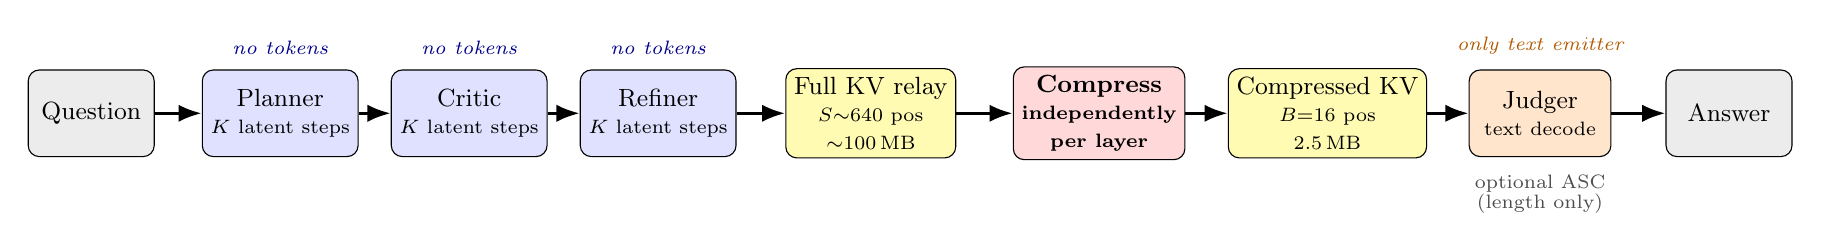
\begin{tikzpicture}[
  font=\small,
  >=Latex,
  box/.style={draw,rounded corners,align=center,minimum height=11mm,inner sep=3pt},
  lat/.style={box,fill=blue!12,minimum width=18mm},
  kv/.style={box,fill=yellow!30,minimum width=20mm},
  cmp/.style={box,fill=red!15,minimum width=20mm,font=\small\bfseries},
  jud/.style={box,fill=orange!20,minimum width=18mm},
  io/.style={box,fill=gray!15,minimum width=16mm}]
  \node[io]  (q)    at (0,0)    {Question};
  \node[lat] (p)    at (2.4,0)  {Planner\\[-1pt]\scriptsize $K$ latent steps};
  \node[lat] (c)    at (4.8,0)  {Critic\\[-1pt]\scriptsize $K$ latent steps};
  \node[lat] (r)    at (7.2,0)  {Refiner\\[-1pt]\scriptsize $K$ latent steps};
  \node[kv]  (full) at (9.9,0)  {Full KV relay\\[-1pt]\scriptsize $S{\sim}640$ pos\\[-1pt]\scriptsize $\sim$100\,MB};
  \node[cmp] (comp) at (12.8,0) {Compress\\[-1pt]\scriptsize independently\\[-1pt]\scriptsize per layer};
  \node[kv]  (small)at (15.7,0) {Compressed KV\\[-1pt]\scriptsize $B{=}16$ pos\\[-1pt]\scriptsize 2.5\,MB};
  \node[jud] (j)    at (18.4,0) {Judger\\[-1pt]\scriptsize text decode};
  \node[io]  (a)    at (20.8,0) {Answer};
  \foreach \x/\y in {q/p,p/c,c/r,r/full,full/comp,comp/small,small/j,j/a}
    \draw[->,very thick] (\x)--(\y);
  \node[above=2pt of p,font=\scriptsize\itshape,text=blue!55!black] {no tokens};
  \node[above=2pt of c,font=\scriptsize\itshape,text=blue!55!black] {no tokens};
  \node[above=2pt of r,font=\scriptsize\itshape,text=blue!55!black] {no tokens};
  \node[above=2pt of j,font=\scriptsize\itshape,text=orange!70!black] {only text emitter};
  \node[below=3pt of j,font=\scriptsize,text=black!70,align=center]
    {optional ASC\\[-1pt]\scriptsize (length only)};
\end{tikzpicture}}
\end{center}

\vspace{0.15em}
\begin{columns}[T,onlytextwidth]
\begin{column}{0.58\textwidth}
\begin{block}{\small Compress($C$; $B{=}16$, $s{=}4$, $r{=}8$) --- every layer}
\vspace{-0.25em}
\begin{enumerate}\scriptsize
  \item Score position $i$:
        $\displaystyle\sigma_i=\sum_{h=1}^{n_{\mathrm{kv}}}\|K_{h,i}\|_2$
        \hfill{\tiny (key-norm; alt: value-norm / recency)}
  \item Keep sinks $\{0,\ldots,s{-}1\}$ \textbf{always}, plus
        $\mathrm{Top}_{B-s}$ by $\sigma$ among $i\ge s$
  \item Sort kept indices ascending; gather those $K/V$ slices
        $\rightarrow$ length $B$
  \item \textbf{evict:} done.\quad
        \textbf{obf:} split dropped into $r$ ordered buckets, mean-pool,
        append $\Rightarrow$ length $B{+}r$
  \item Rebuild HF \texttt{DynamicCache}; Judger attends only to this prefix
\end{enumerate}
\end{block}
\end{column}
\begin{column}{0.40\textwidth}
\begin{center}
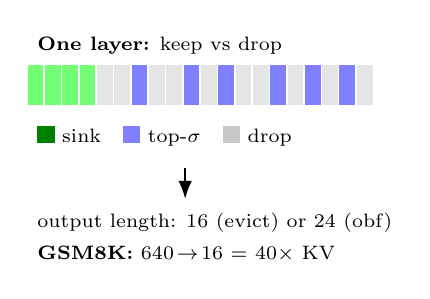
\begin{tikzpicture}[font=\scriptsize,>=Latex]
  \node[anchor=west] at (0,1.0) {\textbf{One layer:} keep vs drop};
  \foreach \i in {0,...,19} {
    \pgfmathsetmacro{\x}{\i*0.22}
    \fill[gray!20] (\x,0.25) rectangle ++(0.20,0.5);
  }
  \foreach \i in {0,1,2,3} {
    \pgfmathsetmacro{\x}{\i*0.22}
    \fill[green!55] (\x,0.25) rectangle ++(0.20,0.5);
  }
  \foreach \i in {6,9,11,14,16,18} {
    \pgfmathsetmacro{\x}{\i*0.22}
    \fill[blue!50] (\x,0.25) rectangle ++(0.20,0.5);
  }
  \node[anchor=west] at (0,-0.15)
    {\textcolor{green!50!black}{\rule{2.2mm}{2.2mm}} sink\quad
     \textcolor{blue!50}{\rule{2.2mm}{2.2mm}} top-$\sigma$\quad
     \textcolor{gray!45}{\rule{2.2mm}{2.2mm}} drop};
  \draw[->,thick] (2.0,-0.55)--(2.0,-0.95);
  \node[anchor=west] at (0,-1.25) {output length: $16$ (evict) or $24$ (obf)};
  \node[anchor=west] at (0,-1.65) {\textbf{GSM8K:} $640\!\to\!16$ $=$ \textbf{$40\times$} KV};
\end{tikzpicture}
\end{center}
\end{column}
\end{columns}
\end{frame}

%------------------------------------------------------------------
\begin{frame}{Setup in one slide}
\begin{center}
\small Question $\to$ Planner $\to$ Critic $\to$ Refiner $\to$
\textbf{relay KV} $\to$ Judger (text) $\to$ Answer
\end{center}
\begin{itemize}
  \item Upstream agents reason in latent space ($K$ steps, no tokens) and grow a shared KV cache.
  \item Only the Judger decodes. Relay is typically $\sim$640--1100 positions / $\sim$100--180\,MB.
  \item Prior finding: relay is largely \textbf{content-insensitive within task} (wrong-question $\approx$ right-question) $\Rightarrow$ should compress.
\end{itemize}
\begin{block}{This week's question}
Can we shrink the relay before the Judger, keep accuracy, and what does that cost?
\end{block}
\end{frame}

%------------------------------------------------------------------
\begin{frame}{Method (what we built)}
\begin{columns}[T]
\begin{column}{0.55\textwidth}
\textbf{Compressor} (\texttt{relay\_compress.py})
\begin{itemize}\small
  \item Keep first $s{=}4$ sinks + top-$(B{-}s)$ by key-norm
  \item Optional OBF: mean-pool evicted mass into $r{=}8$ slots
  \item Modes: full / evict / obf
\end{itemize}
\vspace{0.3em}
\textbf{Harness} (\texttt{exp\_2x2\_relay\_asc.py})
\begin{itemize}\small
  \item Build upstream once $\to$ compress $\to$ batched Judger
  \item Arms A--F + shuffled / none / crosstask
  \item Optional Judger-only ASC (SEAL @ L28)
\end{itemize}
\end{column}
\begin{column}{0.42\textwidth}
\begin{block}{2$\times$2}
\centering\small
\begin{tabular}{lcc}
\toprule
 & no ASC & ASC \\
\midrule
full & A & B \\
obf & C & D \\
\bottomrule
\end{tabular}
\end{block}
\vspace{0.4em}
\footnotesize + E/F = plain evict\\
+ S/N/X diagnostics
\end{column}
\end{columns}
\end{frame}

%------------------------------------------------------------------
\begin{frame}{Headline: GSM8K $\approx 40\times$ at iso-acc}
\begin{center}
\begin{tabular}{lrrr}
\toprule
Arm & Acc & Relay MB & Positions \\
\midrule
A full & 0.817 & 100.0 & $\sim$640 \\
E \textbf{evict @16} & \textbf{0.817} & \textbf{2.5} & \textbf{16} \\
C obf @16 ($+r$) & 0.800 & 3.75 & 24 \\
\bottomrule
\end{tabular}
\end{center}
\vspace{0.4em}
\begin{itemize}
  \item Replicated on seeds \textbf{42 / 123 / 7} ($n{=}60$ each).
  \item Plain eviction matches full; mean-pool OBF backfill not needed here.
  \item Shuffled $\approx$ full (0.800 vs 0.817) --- scaffold story still holds.
\end{itemize}
\begin{alertblock}{Claim-ready}
GSM8K: cut inter-agent KV residency $\sim\!40\times$ with no accuracy loss.
\end{alertblock}
\end{frame}

%------------------------------------------------------------------
\begin{frame}{Harder tasks: thicker residual required}
\begin{columns}[T]
\begin{column}{0.48\textwidth}
\textbf{MATH} (full 0.783)
\begin{center}\small
\begin{tabular}{rrr}
\toprule
Keep $B$ & Acc & vs full \\
\midrule
128 & \textbf{0.800} & $+2$ \\
64 & 0.733 & $-5$ \\
32 & 0.717 & $-7$ \\
\bottomrule
\end{tabular}
\end{center}
\end{column}
\begin{column}{0.48\textwidth}
\textbf{MedQA} (full 0.633)
\begin{center}\small
\begin{tabular}{rrr}
\toprule
Keep $B$ & Acc & vs full \\
\midrule
128 & 0.567 & $-7$ soft \\
64 & 0.517 & $-12$ \\
16--32 & $\sim$0.36 & collapse \\
\bottomrule
\end{tabular}
\end{center}
\end{column}
\end{columns}
\vspace{0.5em}
\begin{block}{Operating rule}
Easy tasks tolerate extreme shrink; harder tasks need keep $\sim$64--128.\\
MedQA with \textbf{no} cache: 0.267 --- presence still matters, thickness matters more.
\end{block}
\end{frame}

%------------------------------------------------------------------
\begin{frame}{Cost: compression overhead is real, but tiny}
\[
t_{\mathrm{e2e}} = t_{\mathrm{upstream}} + t_{\mathrm{compress}} + t_{\mathrm{decode}}
\]
\begin{itemize}
  \item GSM8K keep-16: $\Delta t_{\mathrm{decode}}(C{-}A)\approx -1.05\,\mathrm{s}$,
        $\Delta t_{\mathrm{e2e}}\approx -1.02\,\mathrm{s}$
  \item $\Rightarrow$ $t_{\mathrm{compress}}\approx \textbf{20--25\,ms}$ ($\sim$0.7\% of upstream $\sim$3\,s)
  \item Peak GPU: 36.8 $\to$ 34.1\,GB; relay residency: 100 $\to$ 2.5\,MB
\end{itemize}
\begin{alertblock}{Honest accounting}
$40\times$ is \textbf{relay / Judger-prefix memory}, not ``skip upstream FLOPs.''\\
We still build the full cache once; then shrink it.
\end{alertblock}
\end{frame}

%------------------------------------------------------------------
\begin{frame}{AIME 2024 --- long runs, what we learned}
\begin{itemize}
  \item Full LatentMAS on all 30 AIME problems, up to 8192 output tokens
        (slow: many minutes per $K$, re-run overnight to confirm).
\end{itemize}
\begin{center}
\begin{tabular}{lrrr}
\toprule
Latent steps $K$ & Accuracy & Mean tokens & Mean latency \\
\midrule
0 (Judger only) & 0.53 & 7237 & 178\,s \\
\textbf{10} & \textbf{0.67} & \textbf{5927} & \textbf{146\,s} \\
40 & 0.50 & 6401 & 159\,s \\
\bottomrule
\end{tabular}
\end{center}
\vspace{0.35em}
\begin{itemize}\small
  \item Latent agents help on hard math: $+14$ pts at $K{=}10$ vs Judger-only
        (overnight re-run: $0.67$ vs $0.57$).
  \item More latent steps is not better --- $K{=}40$ falls back to $\sim$Judger-only.
  \item Cutting $K$ does \textbf{not} save wall-clock; Judger length dominates.
\end{itemize}
\begin{block}{\small Compression on AIME}
Tried, but answers often hit the 8192 cap so scores are not trustworthy yet.
Compression claims stay on GSM8K / MATH / MedQA for now.
\end{block}
\end{frame}

%------------------------------------------------------------------
\begin{frame}{Status and proposed next}
\begin{block}{This week}
\begin{itemize}\small
  \item GSM8K: $\sim\!40\times$ relay compression at matched accuracy (3 seeds)
  \item MATH / MedQA: mapped how aggressive we can be before accuracy drops
  \item AIME: confirmed LatentMAS helps at $K{=}10$; compression deferred
\end{itemize}
\end{block}
\begin{block}{Next (pick)}
\begin{enumerate}\small
  \item Put these numbers into the paper draft
  \item Memory--accuracy Pareto figure across keep-budgets
  \item AIME compression only if we re-run without truncation issues
\end{enumerate}
\end{block}
\end{frame}

\end{document}
